%%%%%%%%%%%%%%%%%%%%%%%%%%%%%%%%%%%%%%%%%%%%%%%%%%%%%%%%%%%%%%%%%%%%%%%%%%%%
%% Author: Ming Li
%% Time: 2022-7-18
%% Note: Overleaf版本
%%%%%%%%%%%%%%%%%%%%%%%%%%%%%%%%%%%%%%%%%%%%%%%%%%%%%%%%%%%%%%%%%%%%%%%%%%%%
%%%%%%%%%%%%%%%%%%%%%%%%%%%%%%%%%%%%%%%%%%%%%%%%%%%%%%%%%%%%%%%%%%%%%%%%%%%%
%% Author: Yongtao Zhou <y.t.zhou@foxmail.com>                            %%
%% Time: 2015-4-8                                                         %%
%% Note: 请保留原作者Yongtao Zhou信息,非官方模板。                            %%
%%       最终解释权和所有权利归原作者和数据存储与集群计算实验室所有。               %%
%%%%%%%%%%%%%%%%%%%%%%%%%%%%%%%%%%%%%%%%%%%%%%%%%%%%%%%%%%%%%%%%%%%%%%%%%%%%
\PassOptionsToPackage{quiet}{fontspec}      %% 抑制fontspec警告 
\documentclass[a4paper,oneside,12pt]{book}
\usepackage{amsfonts}
\usepackage{amssymb}
\usepackage{amsmath}
\usepackage{amscd}
\usepackage{amsfonts,eucal}
\usepackage{amsthm}
\usepackage{cite}
\usepackage{bm}
\usepackage[UTF8,fontset=none,heading=true]{ctex}
\usepackage{times}
%% 默认算法环境
\usepackage[linesnumbered,ruled,vlined,boxed,commentsnumbered]{algorithm2e}
%% 常用包
\usepackage{textcomp, gensymb}
\usepackage{graphicx}
\usepackage{url}
\usepackage{multirow}
\usepackage{subfig}
\usepackage{float}
\usepackage{subfig}
\usepackage{array}
\usepackage{amsmath}            %% equation mutilrow align
\usepackage{amsthm}
\usepackage{makecell}
\usepackage{rotating}
\usepackage{booktabs}
\usepackage{algorithm2e}
\usepackage{diagbox}
\usepackage{booktabs}
%% 用geometry宏包设置页边距
\usepackage[top=2.5cm,bottom=2.0cm,left=2.5cm,right=2.5cm]{geometry}
%% 用titlesec宏包设置章节标题
%% 用titletoc宏包设置章页眉页脚和目录的格式
\usepackage[indentafter, pagestyles]{titlesec}
\usepackage{titletoc}
\usepackage{etoolbox}
\usepackage{indentfirst}
\setlength{\parindent}{2em}     %% 2em代表首行缩进两个字符
%% latex超链接
\usepackage{hyperref}

%% 引入书签
\hypersetup{hidelinks,
	colorlinks=true,
	allcolors=black,
	pdfstartview=Fit,
	breaklinks=true
}

%% 用\titleformat命令设置章标题的格式
\titleformat{\chapter}[hang]{\centering\xiaosan\hei}{\thechapter}{1em}{}
\titleformat{\section}[hang]{\sihao\hei}{\thesection}{0.5em}{}
\titleformat{\subsection}[hang]{\xiaosi\hei}{\thesubsection}{0.5em}{}

%% 用\titlespacing或\titlespacing*命令设置标题与四周的距离
\titlespacing{\chapter}{0pt}{*0}{*5}
\titlespacing{\section}{0pt}{*1}{*1}
\titlespacing{\subsection}{0pt}{*0.5}{*0.5}

% %% 重置默认字体--小四
% \renewcommand{\normalsize}{\fontsize{12pt}{14.4pt}\selectfont}

%% 行距倍数
% \renewcommand{\baselinestretch}{1.5}
\renewcommand{\baselinestretch}{1.625}
%% 段落间距
% \setlength{\parskip}{0.3\baselineskip}
\setlength{\parskip}{0\baselineskip}
%% 汉字字距
\renewcommand{\CJKglue}{\hskip 1pt plus 0.08\baselineskip}
%% 重新设置字体大小,行高 = 字体大小 * 1.2
\newcommand{\wuhao}{\fontsize{10.5pt}{12.6pt}\selectfont}          %% 五号字体
\newcommand{\xiaosi}{\fontsize{12pt}{14.4pt}\selectfont}           %% 小四字体
\newcommand{\sihao}{\fontsize{14pt}{16.8pt}\selectfont}            %% 四号字体
\newcommand{\xiaosan}{\fontsize{15pt}{18pt}\selectfont}            %% 小三字体
\newcommand{\sanhao}{\fontsize{16pt}{19.2pt}\selectfont}           %% 三号字体
\newcommand{\xiaoer}{\fontsize{18pt}{21.6pt}\selectfont}           %% 小二字体
\newcommand{\erhao}{\fontsize{22pt}{26.4pt}\selectfont}            %% 二号字体

%% 重设目录设置
\setcounter{tocdepth}{1}
\titlecontents{chapter}[0pt]{\vspace{0pt}\song\xiaosi}
    {\thecontentslabel\hspace{1em}}{}
    {\hspace{0em}\titlerule*[3pt]{$\cdot$}\contentspage}
\titlecontents{section}[0pt]{\vspace{0pt}\hspace{1em}\song\xiaosi}
    {\thecontentslabel\hspace{1em}}{}
    {\hspace{0em}\titlerule*[3pt]{$\cdot$}\contentspage}
\titlecontents{subsection}[0pt]{\vspace{0pt}\song\xiaosi}
    {\thecontentslabel\hspace{1em}}{}
    {\hspace{0em}\titlerule*[3pt]{$\cdot$}\contentspage}

% %% 设置字体大小
% \newcommand{\wuhao}{\fontsize{10.5pt}{12.6pt}\selectfont}        %% 五号字体
% \newcommand{\xiaosi}{\fontsize{12pt}{18pt}\selectfont}           %% 小四字体
% \newcommand{\sihao}{\fontsize{14pt}{21pt}\selectfont}            %% 四号字体
% \newcommand{\xiaosan}{\fontsize{15pt}{22.5pt}\selectfont}        %% 小三字体
% \newcommand{\sanhao}{\fontsize{16pt}{24pt}\selectfont}           %% 三号字体
% \newcommand{\xiaoer}{\fontsize{18pt}{27pt}\selectfont}           %% 小二字体
% \newcommand{\erhao}{\fontsize{22pt}{30pt}\selectfont}            %% 二号字体

% %% 目录设置
% \setcounter{tocdepth}{1}
% \titlecontents{chapter}[0pt]{\vspace{-15pt}\song\xiaosi}
%     {\thecontentslabel\hspace{1em}}{}
%     {\hspace{0em}\titlerule*[3pt]{$\cdot$}\contentspage}
% \titlecontents{section}[0pt]{\vspace{-15pt}\hspace{1em}\song\xiaosi}
%     {\thecontentslabel\hspace{1em}}{}
%     {\hspace{0em}\titlerule*[3pt]{$\cdot$}\contentspage}
% \titlecontents{subsection}[4em]{\vspace{-15pt}\song\xiaosi}
%     {\thecontentslabel\hspace{1em}}{}
%     {\hspace{0em}\titlerule*[3pt]{$\cdot$}\contentspage}

%% 设置中文字体
%% 加载本地中文字体
\setCJKfamilyfont{song}{simsun.ttc}[AutoFakeSlant,AutoFakeBold={2}]     %% 宋体
\newcommand{\song}{\CJKfamily{song}}                                    %% 宋体
\setCJKfamilyfont{hei}{simhei.ttf}[AutoFakeSlant,AutoFakeBold={2}]      %% 黑体
\newcommand{\hei}{\CJKfamily{hei}}                                      %% 黑体
\setCJKfamilyfont{kai}{simkai.ttf}[AutoFakeSlant,AutoFakeBold={2}]      %% 楷体
\newcommand{\kai}{\CJKfamily{kai}}                                      %% 楷体
\setCJKfamilyfont{li}{SIMLI.TTF}[AutoFakeSlant,AutoFakeBold={2}]        %% 隶书
\newcommand{\li}{\CJKfamily{li}}                                        %% 隶书

%%% 如需加载其他中文字体,可以从网上或者C:\Windows\Fonts复制字体文件到根目录下加载即可。
%% \newcommand{\fs}{\CJKfamily{fs}}        %% 仿宋
%% \newcommand{\you}{\CJKfamily{you}}      %% 幼圆
\setCJKmainfont{simsun.ttc}[AutoFakeSlant,AutoFakeBold={2}]

%% 设置英文字体
\RequirePackage{xltxtra}                %% \XeTeX Logo
\setmainfont{Times New Roman}
\setsansfont{Arial}
\setmonofont{Times New Roman}

\newcommand*\aap{Astronomy \& Astrophysics}
\let\astap=\aap
\newcommand*\aaps{American Association of Pharmaceutical Scientists}
\newcommand*\aj{Astronomical Journal}
\let\applopt\ao
\newcommand*\apj{Astrophysical Journal}
\newcommand*\apjl{Astrophysical Journal Letters}
\let\apjlett\apjl
\newcommand*\apjs{Astronomical Journal Supplementary Series}
\let\apjsupp\apjs
\newcommand*\aplett{Astrophys.~Lett.}
\newcommand*\apspr{Astrophys.~Space~Phys.~Res.}
\newcommand*\apss{Astrophysics and Space Science}
\newcommand*\caa{Chinese Astron. Astrophys.}
\newcommand*\cjaa{Chinese J. Astron. Astrophys.}
\newcommand*\icarus{Icarus}
\newcommand*\mnras{MNRAS}
\newcommand*\na{New A}
\newcommand*\nar{New A Rev.}
\newcommand*\nat{Nature}
\newcommand*\pasa{Publications of The Astronomical Society of Australia}
\newcommand*\pasj{Publications of The Astronomical Society of Japan}
\newcommand*\pasp{Publications of The Astronomical Society of The Pacific}
\newcommand*\planss{Planetary and Space Science}
\newcommand*\ssr{Space Science Reviews}

%% 设置页眉页脚
\newpagestyle{main}[\wuhao]{
\sethead{}{\pageHeaderTitle}{}
\setfoot{}{\thepage}{} \setheadrule{0.05pt}}\pagestyle{main}

%% 重置目录的名称
\renewcommand{\contentsname}{目\qquad 录}

%% 算法环境的重置
\renewcommand{\algorithmcfname}{算法}
\SetKwInput{KwData}{输入}
\SetKwInput{KwResult}{输出}

%% 图表重置
%% 设置公式的编号为短杠形式
\renewcommand\theequation{%
\thechapter-\arabic{equation}}
%% 设置图, 表的编号为短杠形式
\renewcommand\thefigure{\arabic{chapter}-\arabic{figure}}
\renewcommand\thetable{\arabic{chapter}-\arabic{table}}
%% 设置控制标签与标题之间的间隔形式
\renewcommand{\figurename}{图}
\renewcommand{\tablename}{表}
\usepackage[labelsep=space]{caption}

%% 中文和英文之间加入波浪符“~”,或“ \ ”
%% 例如:中文~abc~中文
%% 中英文混排的时候是用中文标点还是英文标点呢?
%% 这并没有统一的规范。不过比较合理也比较通行的做法是
%% 中文后用中文标点,英文后用英文标点
%% 一般数学文章习惯用全角的实心句点作为中文句号
%% 全角的中文括号看起来不太好看,可以统一使用英文的括号
%% 左括号前面和右括号后面最好加上波浪符“~”
%% 在缩写词后面加上波浪符“~”,如 pp.~100, cf.~something
%% 定义符合中文习惯的定理环境
\newtheoremstyle{mythm}{1.5ex plus 1ex minus .2ex}{1.5ex plus 1ex minus .2ex}{\kai}{\parindent}{\song\bfseries}{}{1em}{}
\theoremstyle{mythm}
\newtheorem{thm}{定理~}[chapter]
\newtheorem{lem}{引理~}
\newtheorem{prop}{命题~}
\newtheorem{cor}{推论~}
\newtheorem{defn}{定义~}
\newtheorem{conj}{猜想~}
\newtheorem{exmp}{例~}
\newtheorem{rem}{注~}
\newtheorem{notation}{记号~}

\newtheoremstyle{specthm}{1.5ex plus 1ex minus .2ex}{1.5ex plus 1ex minus .2ex}{\kai}{\parindent}{\song\bfseries}{}{1em}{\thmnote{#3}}
\theoremstyle{specthm}
\newtheorem{sthm}[thm]{}
%% 例如:
%% \begin{sthm}[定理~\thethm~(存在性定理)]
%% 定理内容
%% \end{sthm}
%% 定义符合中文习惯的证明环境
\makeatletter
\renewenvironment{proof}[1][\proofname]{\par
    \pushQED{\qed}%
    \normalfont \topsep6\p@\@plus6\p@ \labelsep1em\relax
    \trivlist
    \item[\hskip\labelsep\indent
        \bfseries #1]\ignorespaces
}{%
    \popQED\endtrivlist\@endpefalse
}
\makeatother


%% 将文献引用作为上标出现
\makeatletter
\def\@cite#1#2{\textsuperscript{[{#1\if@tempswa , #2\fi}]}}
\makeatother

%% 修改图表目录的指引线距离
\makeatletter
\def\@dotsep{1} % 默认是4.5,就是点之间距离为4.5mu。可以改成2
\makeatother

\renewcommand{\proofname}{证明}
%% proof环境会自动在证明最后一行的最右边加上一个证明结束符
%% 默认为空心方块,可以重新定义 \qedsymbol 来修改它
%% 需要注意的是,当证明以一个独立公式结束时
%% 证明结束符会出现在下一行的最右边,而不是在公式的同一行上
%% 这不合乎习惯。这时只要在公式环境内加上 \qedhere 即可

% Added Library
% Added Library
\usepackage{xcolor}


\begin{document}
%% 参考文献格式重置,重置参考文献的名称
\def\thebibliography#1{\chapter*{参\ 考\ 文\ 献}
    \addcontentsline{toc}{chapter}{参考文献}
    \thispagestyle{main}
    \list
    {[\arabic{enumi}]}{\settowidth\labelwidth{[#1]}\leftmargin\labelwidth
    \advance\leftmargin\labelsep
    \usecounter{enumi}}
    \def\newblock{\hskip .11em plus .33em minus .07em}
    \sloppy\clubpenalty4000\widowpenalty4000
    \sfcode`\.=1000\relax
}

%% 修改参考文献条目之间的竖直方向上的距离
\patchcmd{\thebibliography}{\leftmargin\labelwidth}{\leftmargin\labelwidth\addtolength\itemsep{-8pt}}{}{}

%% 前言
%%-------------------这里定义论文相关信息--------------------
%% 作者名字
\newcommand{\authorName}{作者姓名(若是同等学力人员请注明“同等学力申请”,若是港澳台侨及海外留学生请注明申请人生源地)}
%% 论文题目
\newcommand{\titleCn}{暨南大学硕士学位论文Overleaf模板v1.0}
\newcommand{\titleEn}{论文英文题目}
%% 导师及其职称
\newcommand{\tutor}{导师姓名\ 导师学位\ 导师职称}
%% 学科、专业名称
\newcommand{\disciplineName}{学科\ 专业}
%% 学位类型
\newcommand{\degreeType}{(学术学位/专业学位)}
%% 论文提交时间
\newcommand{\commitDate}{2023\ 年\ 6\ 月}
%% 论文答辩时间
\newcommand{\replyDate}{2023\ 年\ 6\ 月}
%% 答辩委员会主席
\newcommand{\programCoChairs}{委员会主席\ 职称}
%% 论文评阅人
\newcommand{\Reviewer}{评阅人名字\ 职称}
%% 学位论文授予单位日期
\newcommand{\grantDate}{2023\ 年\ 6\ 月}
\newcommand{\schoolName}{暨南大学}
\newcommand{\pageHeaderTitle}{暨南大学硕士学位论文}

%%-------------------这是标题页--------------------
\begin{titlepage}
\begin{flushleft}
    \zihao{-1}\li\textbf{暨南大学硕士学位论文}
\end{flushleft}
\begin{flushleft}
\vspace{25pt}
题名: \titleCn \\
Title: \titleEn    \\[25pt]
作者姓名:\authorName \\[25pt]
指导教师姓名
及学位、职称:\tutor \\[25pt]
学科、专业名称:\disciplineName \\[25pt]
学位类型:\degreeType \\[25pt]
论文提交时间:\commitDate \\[25pt]
论文答辩时间:\replyDate \\[25pt]
答辩委员会主席:\programCoChairs \\[25pt]
论文评阅人:\Reviewer\\[25pt]
学位授予单位日期:\grantDate\\[25pt]
\end{flushleft}
\end{titlepage}

\begin{titlepage}
\begin{center}
    \zihao{2}\song\textbf{独~创~性~声~明}
\end{center}
\par 本人声明所呈交的学位论文是本人在导师指导下进行的研究工作及取得的研究成果。除了文中特别加以标注和致谢的地方外,论文中不包含其他人已经发表或撰写过的研究成果,也不包含为获得\kai{\zihao{3}\textbf{\underline{~~~~\schoolName~~~~}}}\song 或其他教育机构的学位或证书而使用过的材料。与我一同工作的同志对本研究所做的任何贡献均已在论文中作了明确的说明并表示谢意。\\[25pt]
\par 学位论文作者签名:\hspace{115pt}签字日期:~~~~~~年~~~~~~月~~~~~~日\\[25pt]
\begin{center}
    \song\zihao{2}\textbf{学位论文版权使用授权书}
\end{center}
\par 本学位论文作者完全了解\kai{\zihao{3}\textbf{\underline{~~~~~\schoolName~~~~~}}}\song 有关保留、使用学位论文的规定,有权保留并向国家有关部门或机构送交论文的复印件和磁盘,允许论文被查阅和借阅。本人授权\kai{\zihao{3}\textbf{\underline{~~~~\schoolName~~~~}}}\song 可以将学位论文的全部或部分内容编入有关数据库进行检索,可以采用影印、缩印或扫描等复制手段保存、汇编学位论文。
\par (保密的学位论文在解密后适用本授权书)\\[25pt]
\begin{flushleft}
学位论文作者签名:\hspace{135pt}导师签名:\\
签字日期:~~~~~~年~~~~~~月~~~~~~日\hspace{95pt}签字日期:~~~~~~年~~~~~~月~~~~~~日\\
学位论文作者毕业后去向:\\
工作单位:\hspace{185pt}电话:\\
通讯地址:\hspace{185pt}邮编:\\
\end{flushleft}
\end{titlepage}



%% 摘要
\frontmatter \pagenumbering{Roman}  %% 采用大写罗马数字,缺省时为小写的

\chapter*{摘\texorpdfstring{\qquad}{} 要}\addcontentsline{toc}{chapter}{摘要}
\thispagestyle{main}
%% 加星号*的章节默认是不加入目录中的
%% 这个命令\addcontentsline{toc}{chapter}{摘\qquad 要}
%% 使其也加到目录中,且显示为“摘    要”,以下类似
%% 每一章第一页默认是没有页眉的,这里的命令\thispagestyle{main}
%% 使这一页也有页眉,以下类似

\par 本模板由Yongtao Zhou制作,Ming Li二次修改,非官方模板,请选择性使用,最终解释权和所有权归原作者所有。仅供个人学习、学术交流使用,可以随意修改,保留原作者信息即可$\wedge\_\wedge$。
\par 如果您在使用中有建议和发现任何的bug,可以随时联系我修改
$$li-ming96@foxmail.com$$
% \par 本项目地址:https:$//$github.com$/$ytZhou$/$JNUMasterThesis
\par PS:注意做好项目备份,避免造成不必要的损失,由于自己误操作造成的损失作者概不负责和理会。

%%保留下面一行留白

\bigskip
\noindent {\bfseries 关键词:} 模板;非官方;学术交流;项目备份


%\chapter*{The Subject of Undergraduate Graduation Project (Thesis) of DUT\ \vspace{4ex} {\bfseries Abstract}}\addcontentsline{toc}{chapter}{Abstract}
\chapter*{\bfseries ABSTRACT}\addcontentsline{toc}{chapter}{ABSTRACT}
\thispagestyle{main}

\par With the advent of huge amounts of data and the age of big data, digital TV、 digital
camera、 web、 video、 large shopping site, etc, dramatically accelerated the growth of the data. In recent years, the global total data is growing at a speed more than 60\% every year, the data need to backup and archive has brought great pressure on backup system. Deduplication technology has effectively reduced the storage cost by removing redundant data and reducing the actual use of storage capacity.
%%保留下面一行留白

\bigskip
\noindent {\bfseries Key Words: }Key Word 1; Key Word 2; Key Word 3


%% 生成目录
\tableofcontents
\thispagestyle{main}

%% 重置图/表目录(取消不同章之间的间隔)
\begingroup
	\renewcommand*{\addvspace}[1]{}
	\newcommand{\loflabel}{图} 
	\renewcommand{\numberline}[1]{\loflabel~#1\hspace*{1em}}
    \renewcommand{\listfigurename}{图目录}
	\listoffigures
	
	\newcommand{\lotlabel}{表}
	\renewcommand{\numberline}[1]{\lotlabel~#1\hspace*{1em}}
    \renewcommand{\listtablename}{表目录}
	\listoftables
\endgroup
% %%图目录
% \listoffigures
% \thispagestyle{main}
% %%表格目录.
% \listoftables
% \thispagestyle{main}

%% 正文
\mainmatter
%% 设置章节格式(一倍行距为字体大小 × 1.297(1.3) × 1.25)
\ctexset{chapter={
        name = {},
        number = {\arabic{chapter}},
        format = {\bfseries \sffamily \hei \centering \zihao{-3}},
        beforeskip = 15pt,
        afterskip = 25pt,
        fixskip = true,
        aftername = ~~~~,
    }
}
%% 设置一级章节格式
\ctexset{section={
        format = {\bfseries \sffamily \hei \raggedright \zihao{4}},
        beforeskip = 25pt,
        afterskip = 20pt,
        fixskip = true,
    }
}
%% 设置二级标题格式 
\ctexset{subsection={
        format = {\bfseries \sffamily \hei \raggedright \zihao{-4}},
        beforeskip = 20pt,
        afterskip = 20pt,
        fixskip = true,
    }
}
%% 设置三节标题格式
\ctexset{subsubsection={
        format = {\bfseries \sffamily \hei \raggedright \zihao{-4}},
        beforeskip = 20pt,
        afterskip = 20pt,
        fixskip = true,
    }
}

%% 论文正文部分,在chaps.tex内编辑
%% 引入正文章节
\chapter{绪论}\thispagestyle{main}

\section{课题背景}

\par 我们正处在海量数据和大数据的时代,数字电视、摄像机以及其他通讯技术的出现正快速的加剧着数据的增长。据 IDC(国际数据中心International Data Center)统计,2007年数字内容总量第一次超过了全球存储总容量,并且每年数据总量以指数的速度不断增长。数据的爆炸性的增长给大型企业的数据中心带来了较大的压力,以不断扩大甚至扩建数据中心的方式并不能有效的缓解需要存储的数据的增长速度。同时,随着科技的快速发展和信息化的全面普及,数据对于企业甚至国家越来越重要,对于银行和互联网等公司,数据是它们赖以生存的根本,决定着未来的命运。

\par 但是,由于种种未知的原因,人们无法预知或者避免数据的丢失和损坏。例如恐怖事件、系统故障、人为操作、自然灾害、黑客攻击、计算机病毒等各种因素,时刻威胁着大量对企业和国家至关重要的数据。在1993 年,美国世贸中心由于恐怖袭击发生爆炸。在爆炸前,大约有 350 家企业在该大楼中办公,然而一年后,世贸大楼的公司只剩下了150 家,其余的 200 家公司由于无法获取原有的重要数据而被迫倒闭。 根据Gartner Group 的数据表明,企业数据灾难导致很多公司停止运营,其中2/5的公司无法再重新恢复,剩下的也有1/3在两年内相继宣告破产。

\par 重复数据删除技术是一种新型的高级的数据压缩方式,它通过识别出重复的数据部分,删除冗余的部分,是一种更有效的节省磁盘空间的方法。研究发现,在数据备份系统中所存储的数据中有高达60\%的数据是冗余的,而且这一比例会逐渐增加。

\par 因此,基于重复数据删除技术的备份系统,对于节省磁盘空间、减少网络带宽、缩短恢复窗口期等有很重要的理论意义和实际意义。

\section{国内外研究现状}

\par 重复数据删除技术作为一种有效的数据压缩方法被存储界列为十大存储热门技术之一,最早是由美国的\ \ Data Domain\ \ 公司提出来的。在数据备份和归档领域得到了广泛的运用,由于基于重复数据删除技术的备份系统能够取得较好的压缩率以及性能,以及相应的带来的节省带宽、降低成本等效益,重复数据删除技术越来越受到学术界和工业界的关注,成为存储界的一大新兴技术热点,并在高校和企业广泛研究和应用,并且取得了一系列的成果。

\chapter{Latex部分代码示例}\thispagestyle{main}

\section{图片}

\subsection{单张图片示例}

\par \textbf{注意,图片的标题在下面。}

\begin{figure}[!ht]
    \centering
    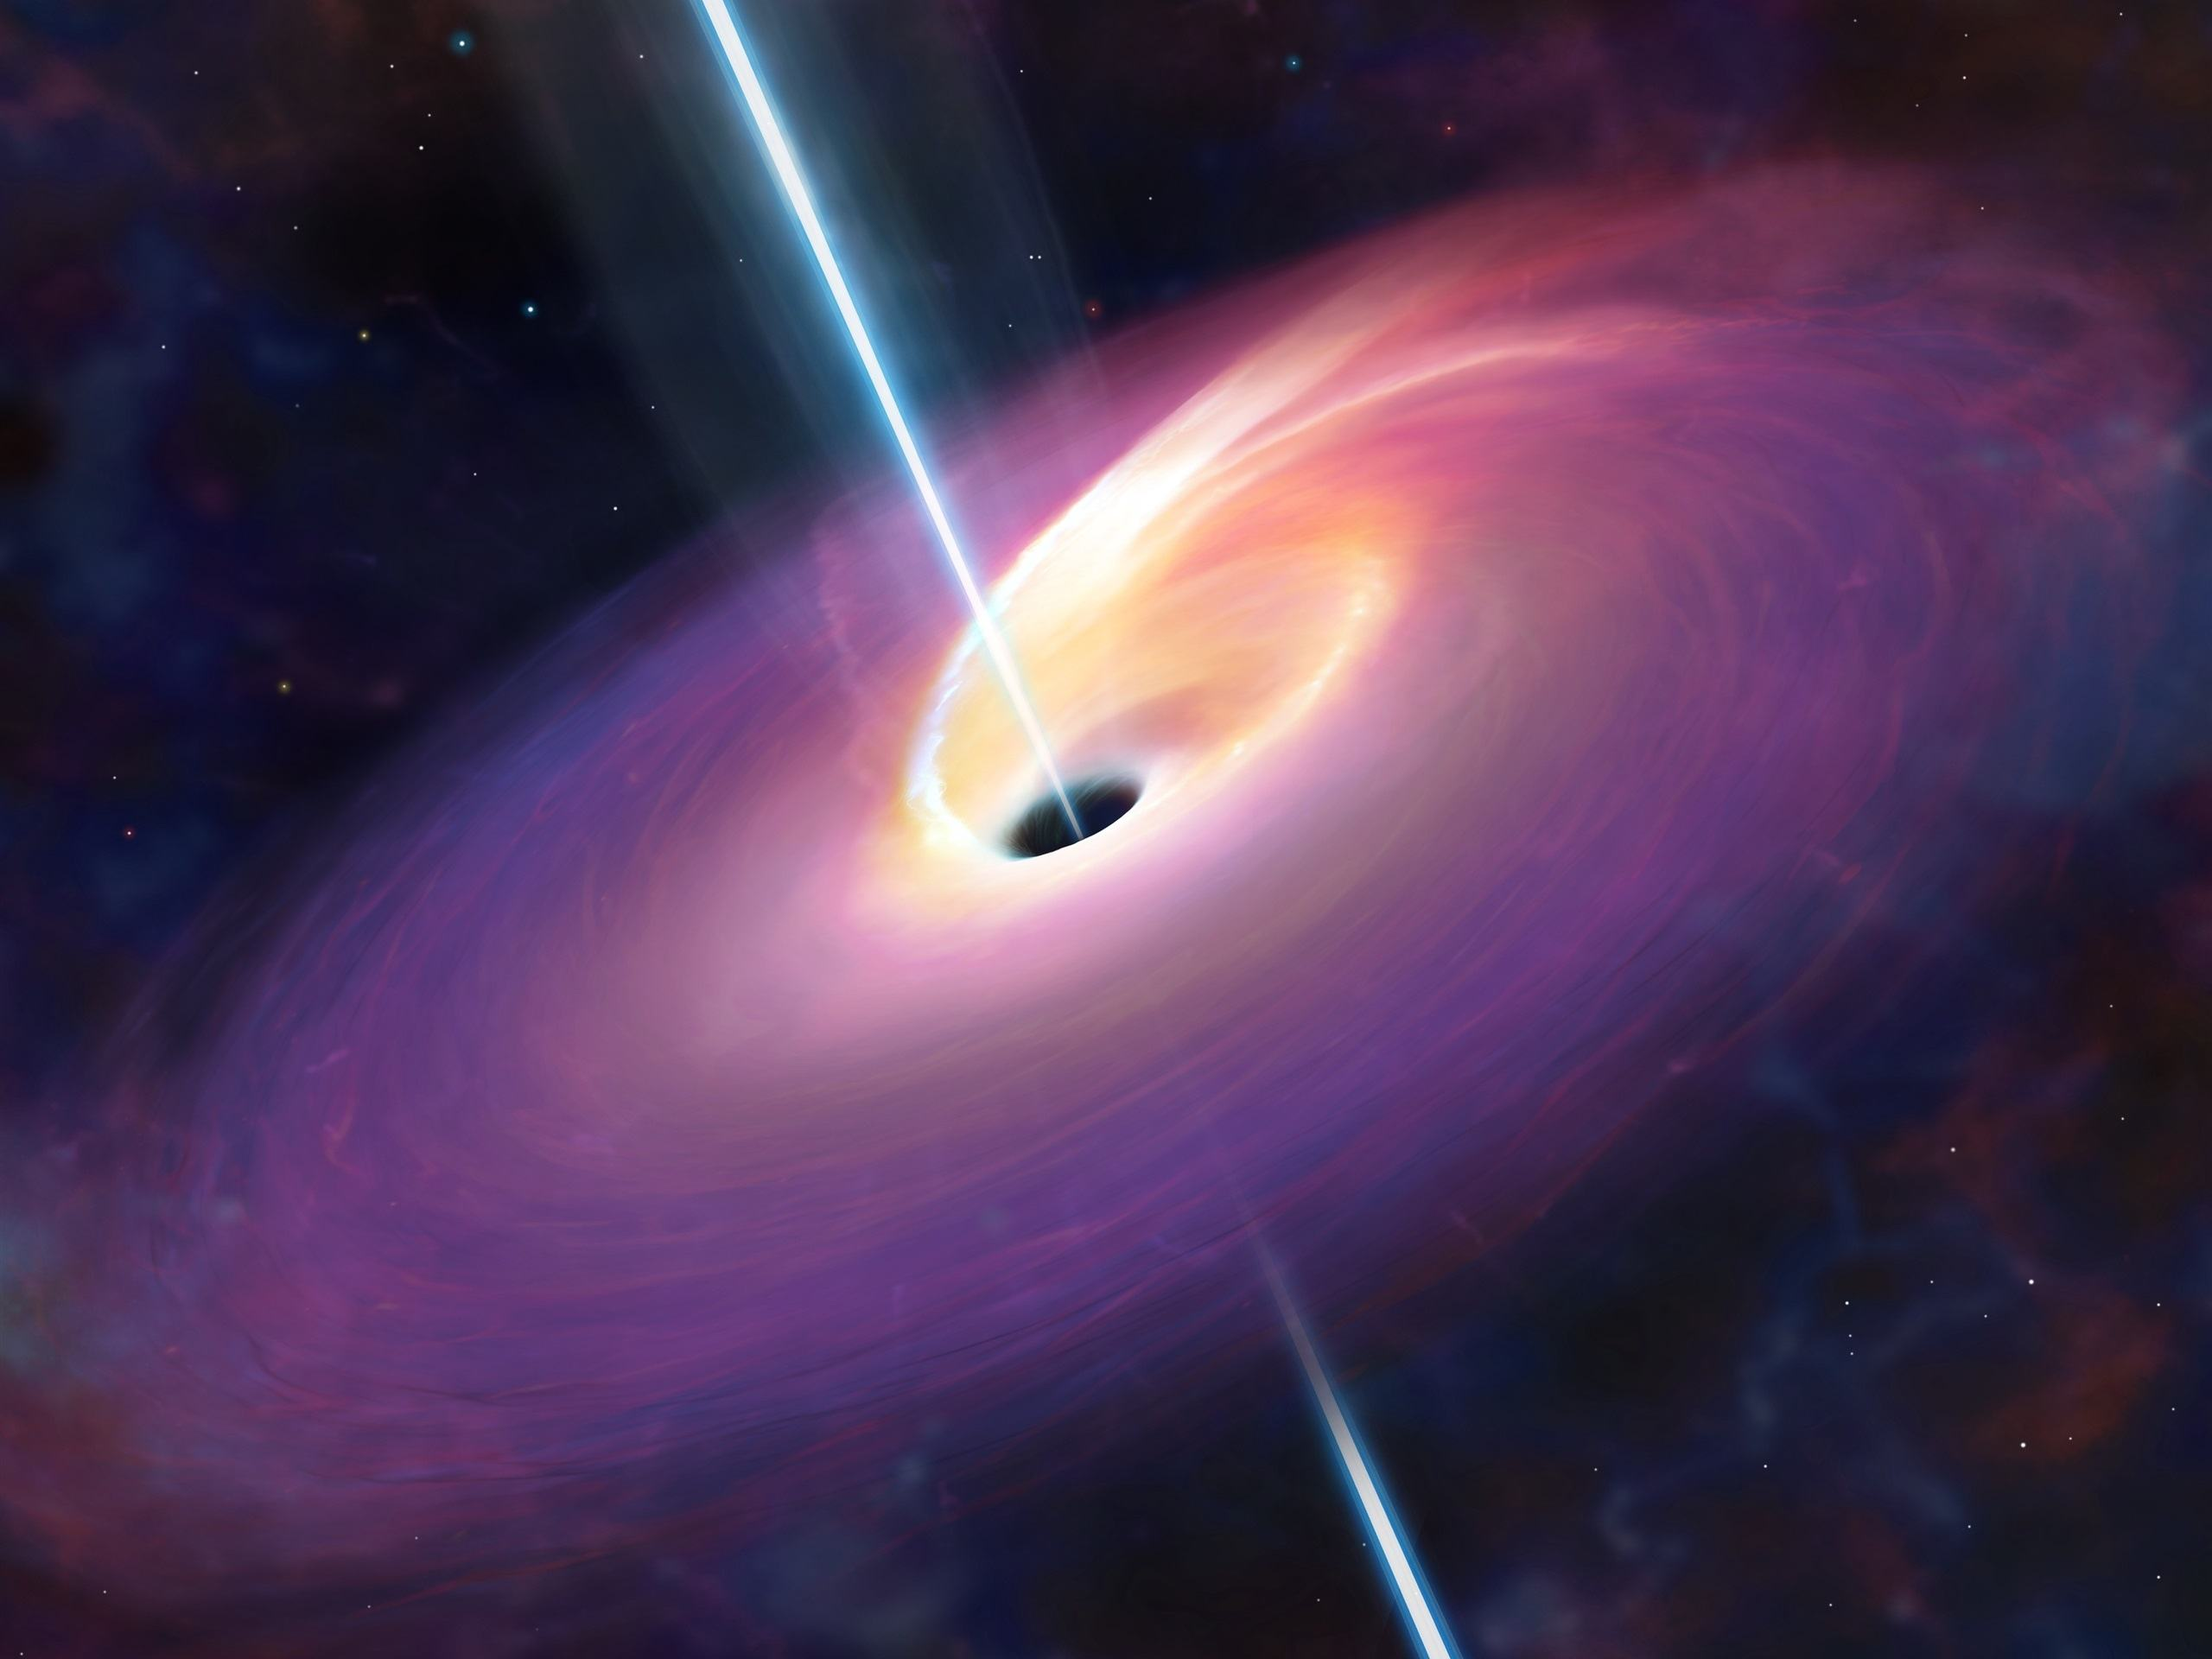
\includegraphics[width=2.5in]{images/blackhole.jpeg}
    \caption{黑洞}
    \label{fig:blackhole1}
\end{figure}
图\ref{fig:blackhole1}是单个黑洞图片。

\subsection{多张图片示例}

\begin{figure*}[!ht]
    \centering
    \subfloat[黑洞1。]{
        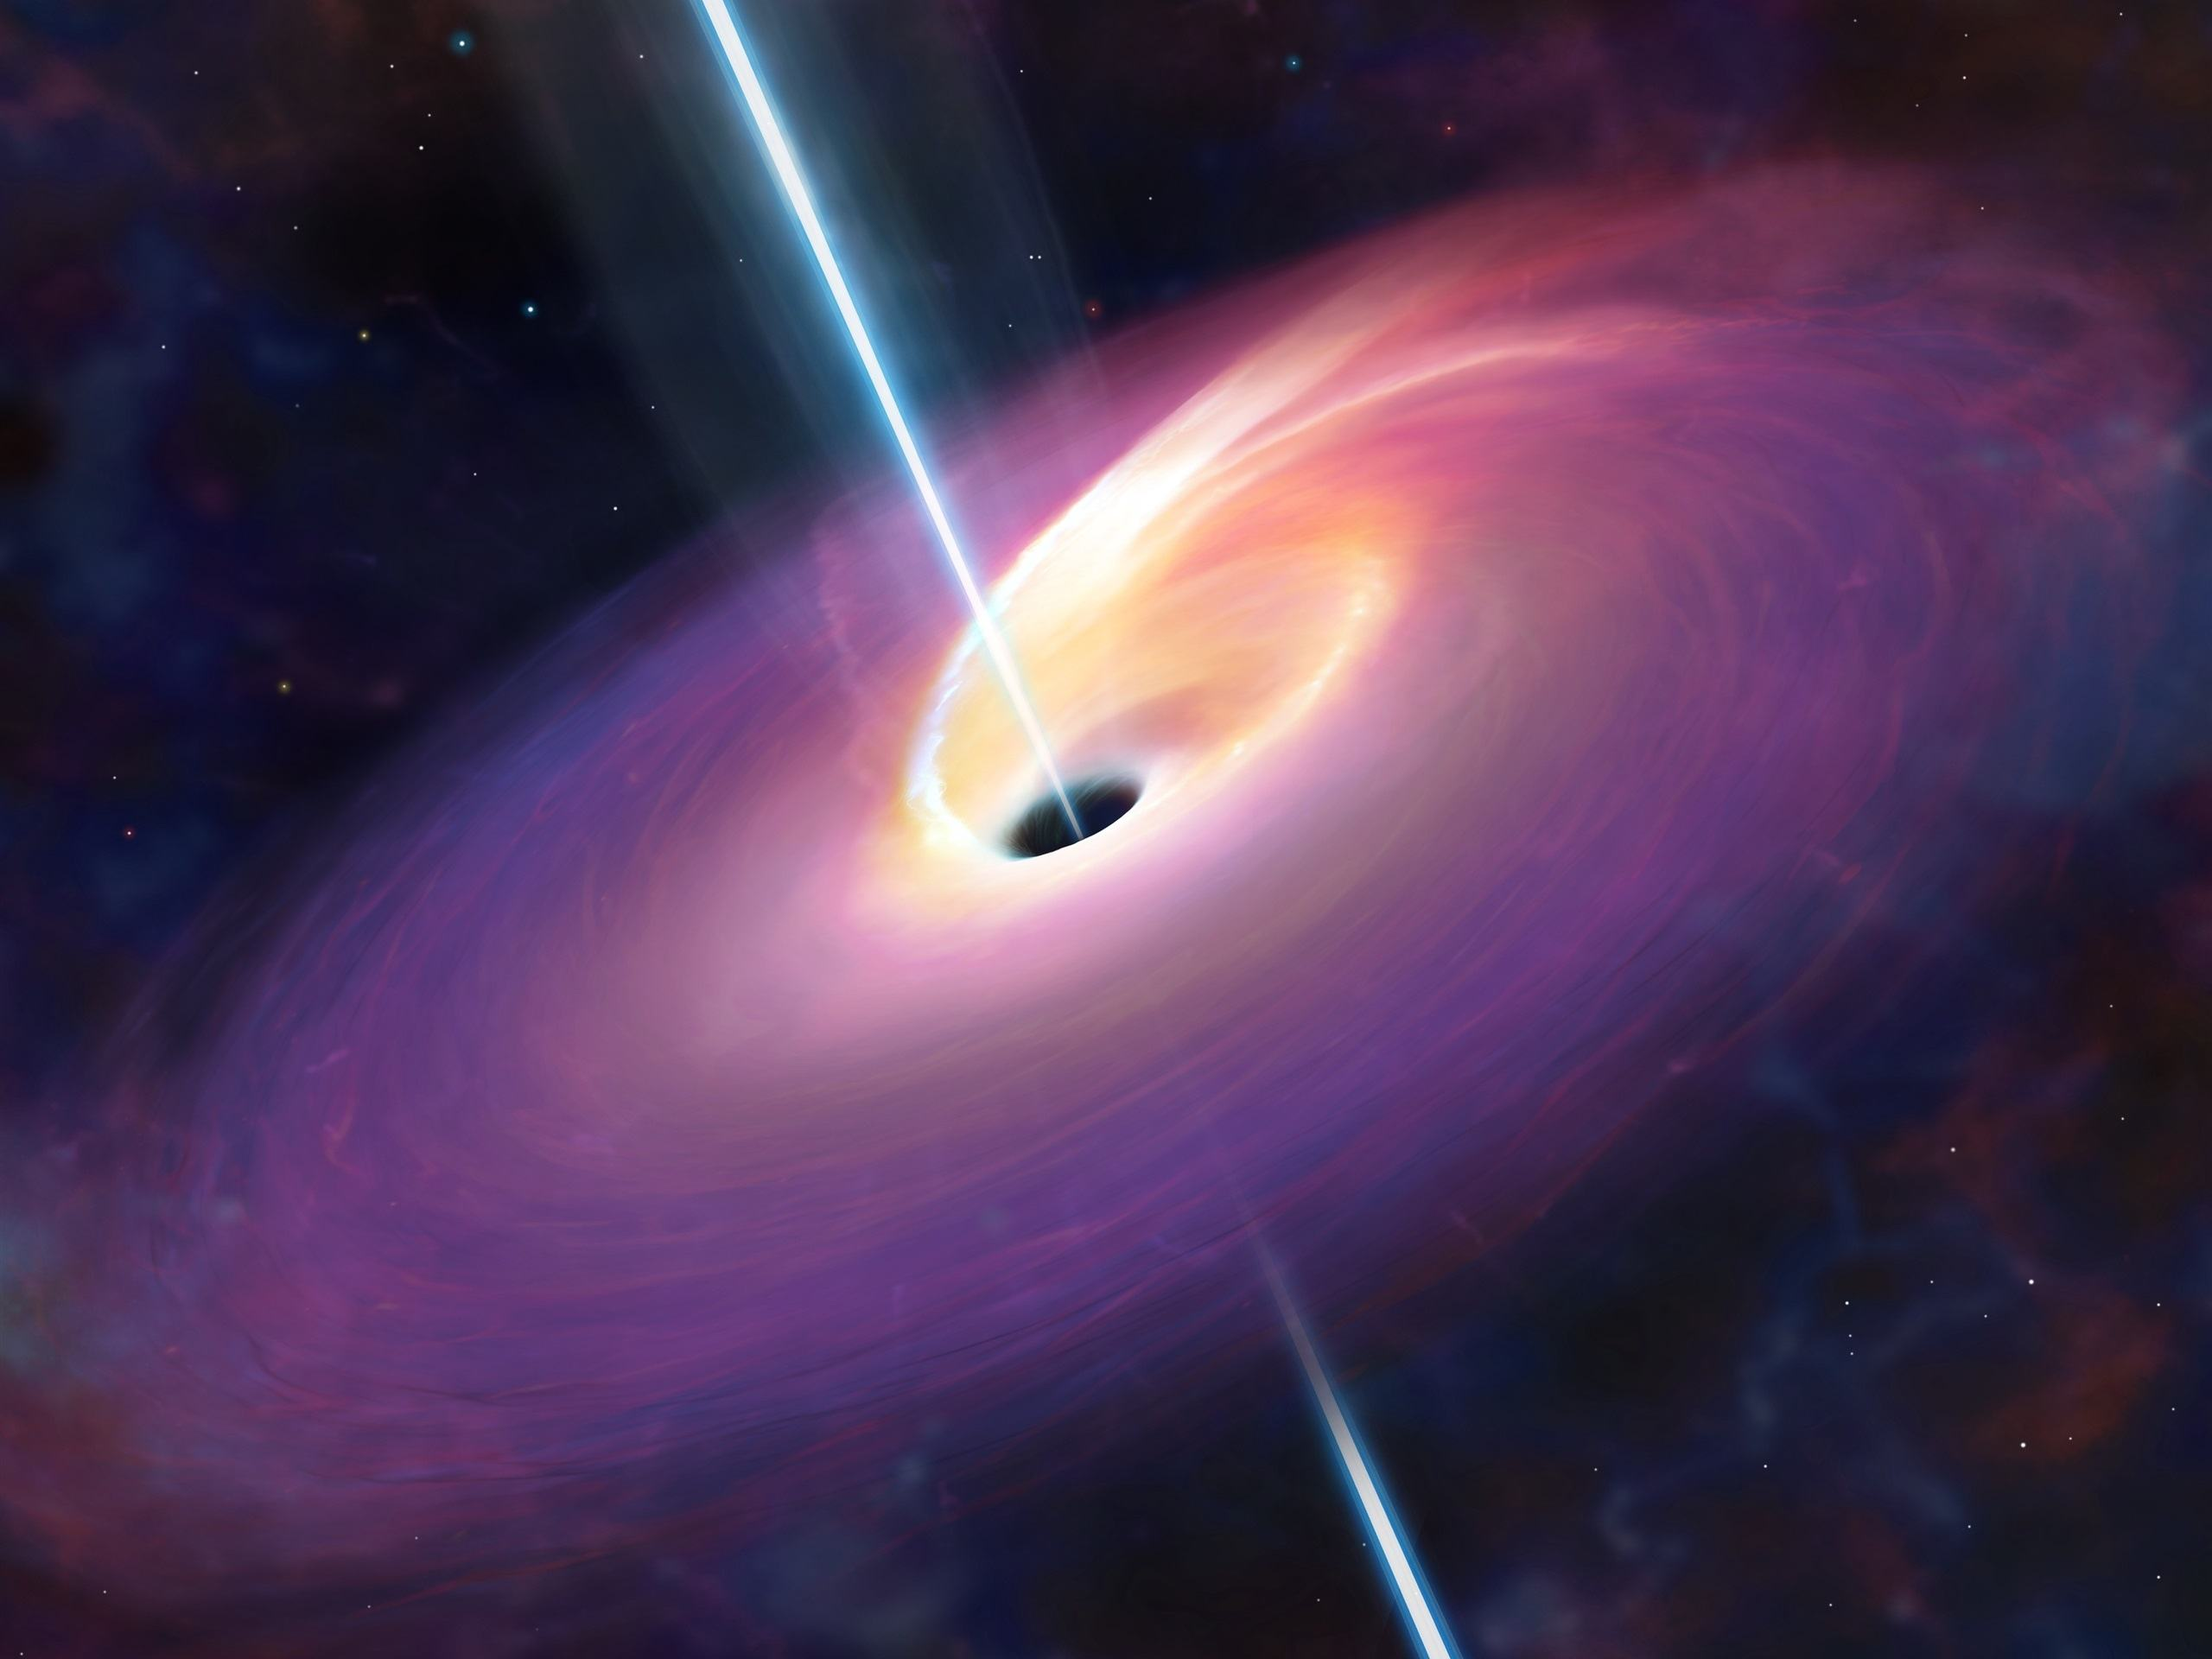
\includegraphics[width = 0.45\textwidth]{images/blackhole.jpeg}
    }
    \hfill
    \subfloat[黑洞2。]{
        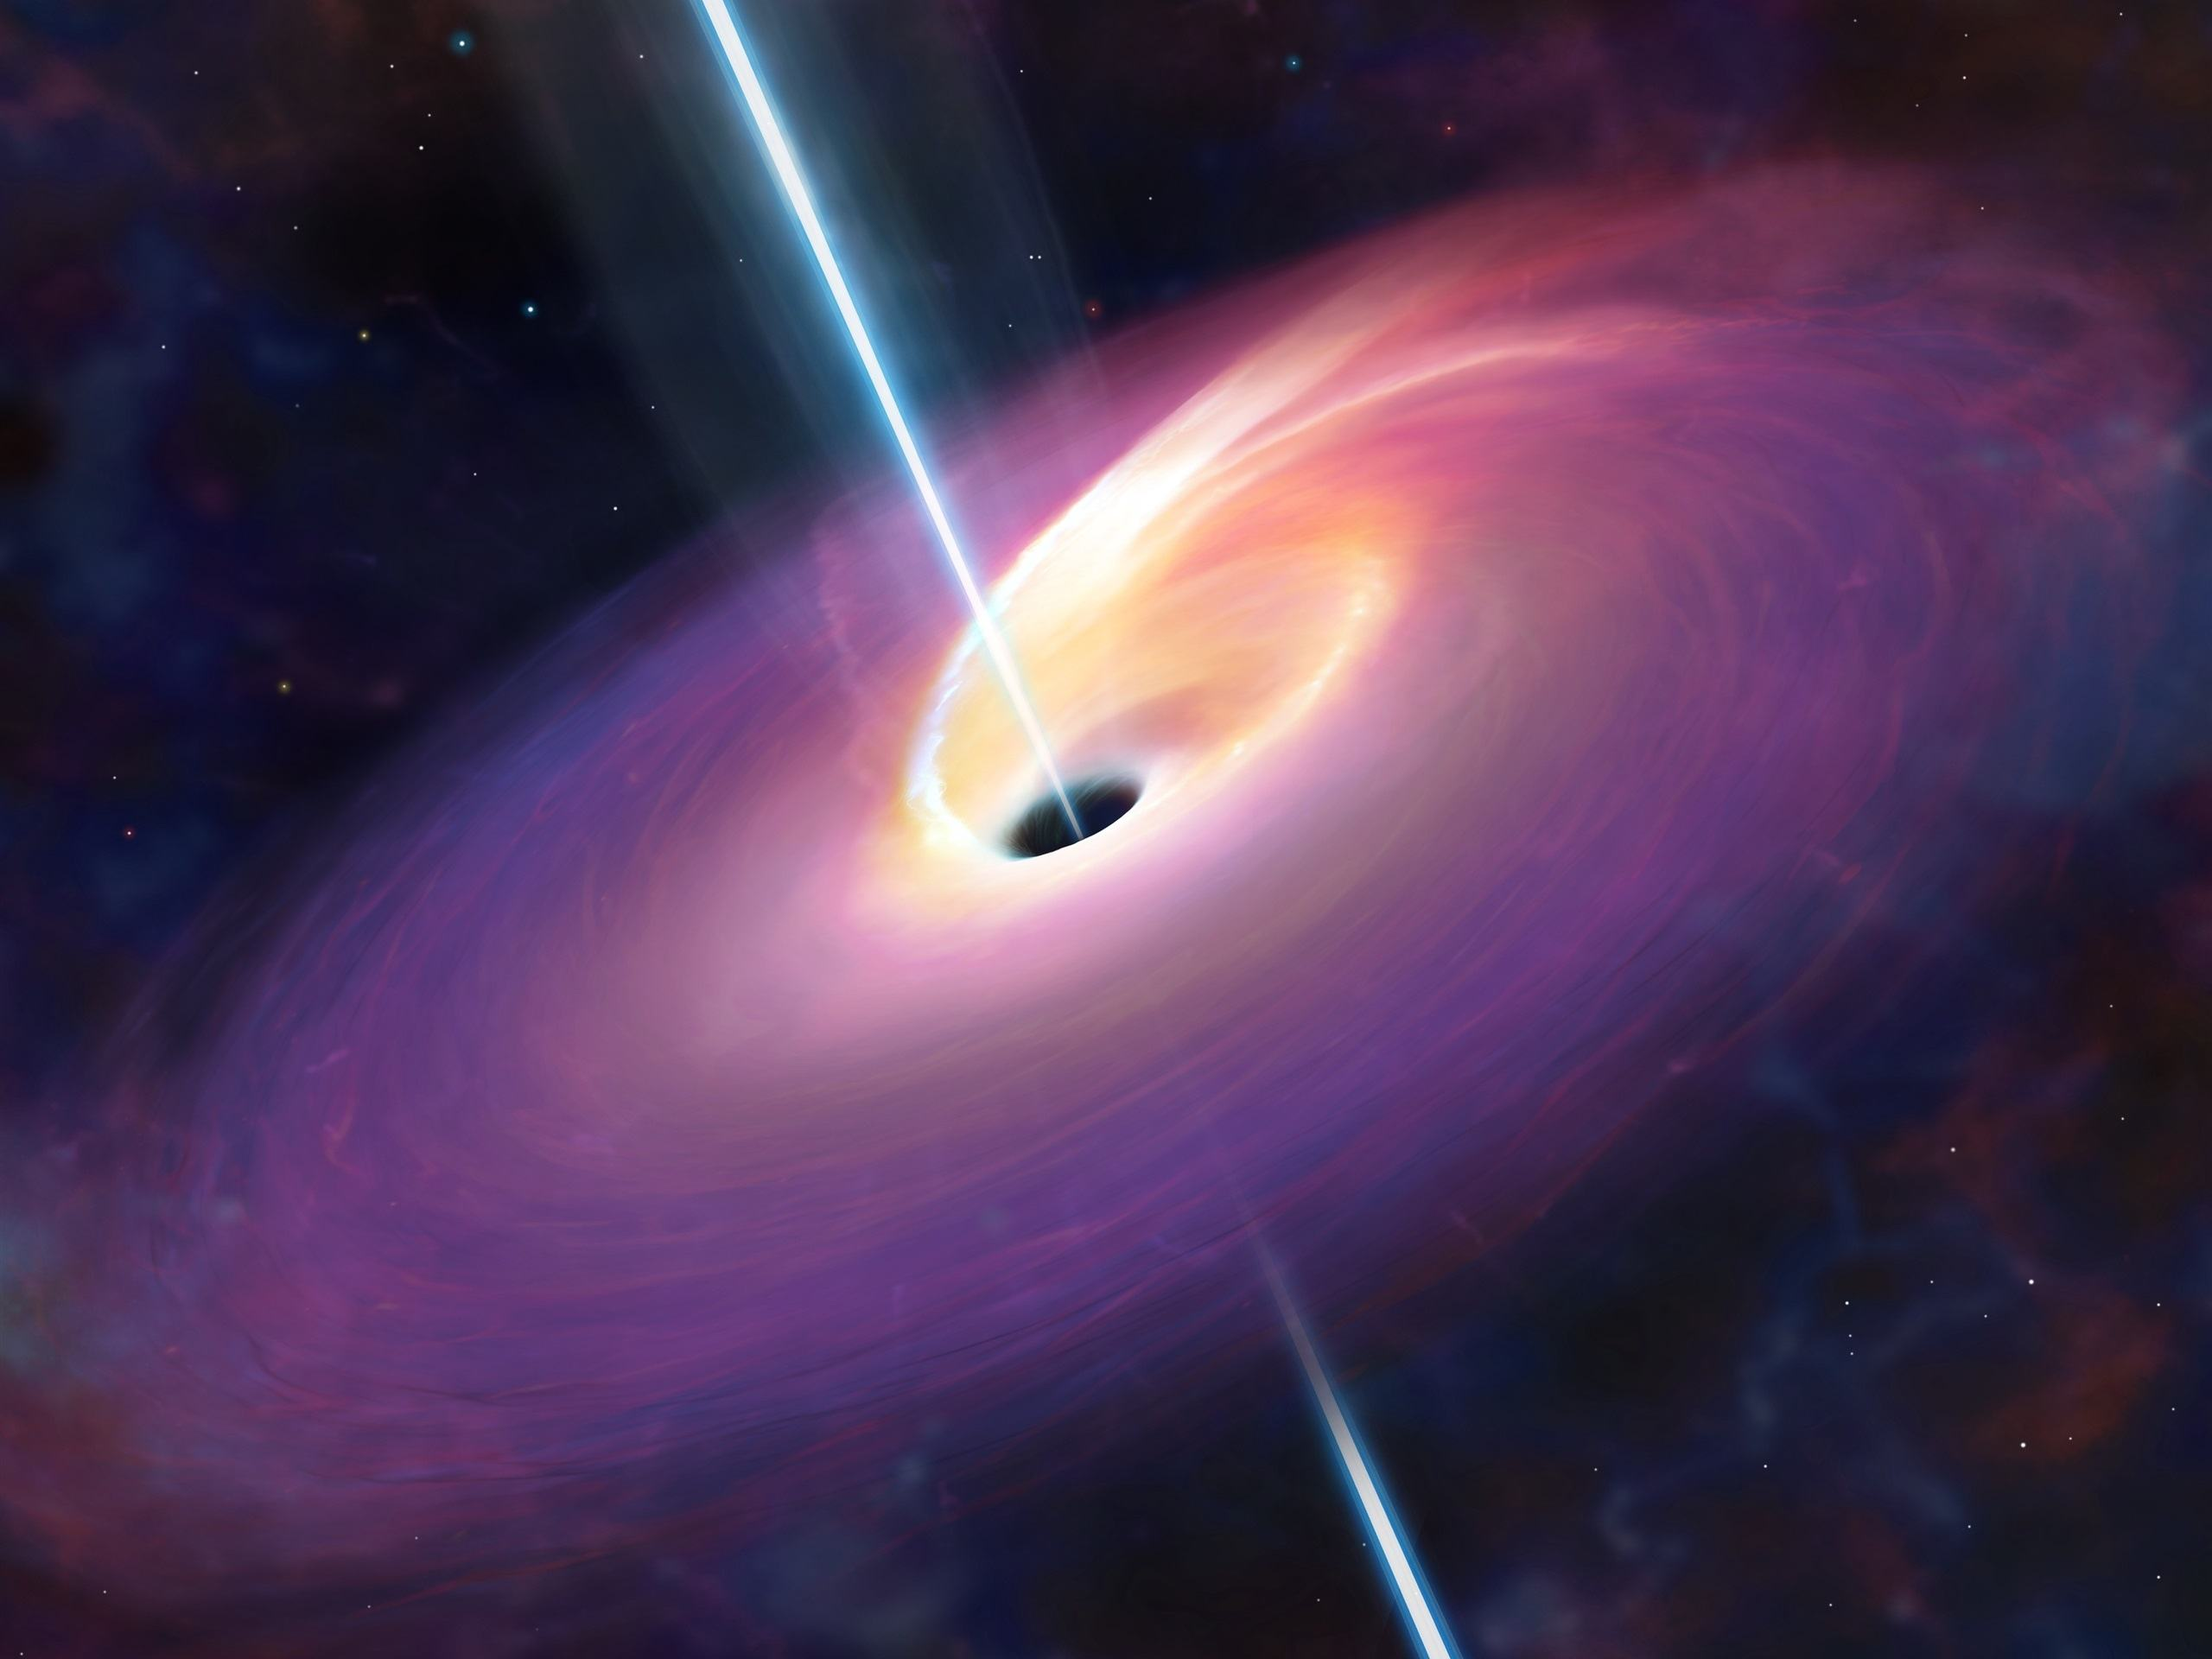
\includegraphics[width = 0.45\textwidth]{images/blackhole.jpeg}
    }
    \\
    \subfloat[黑洞3。]{
        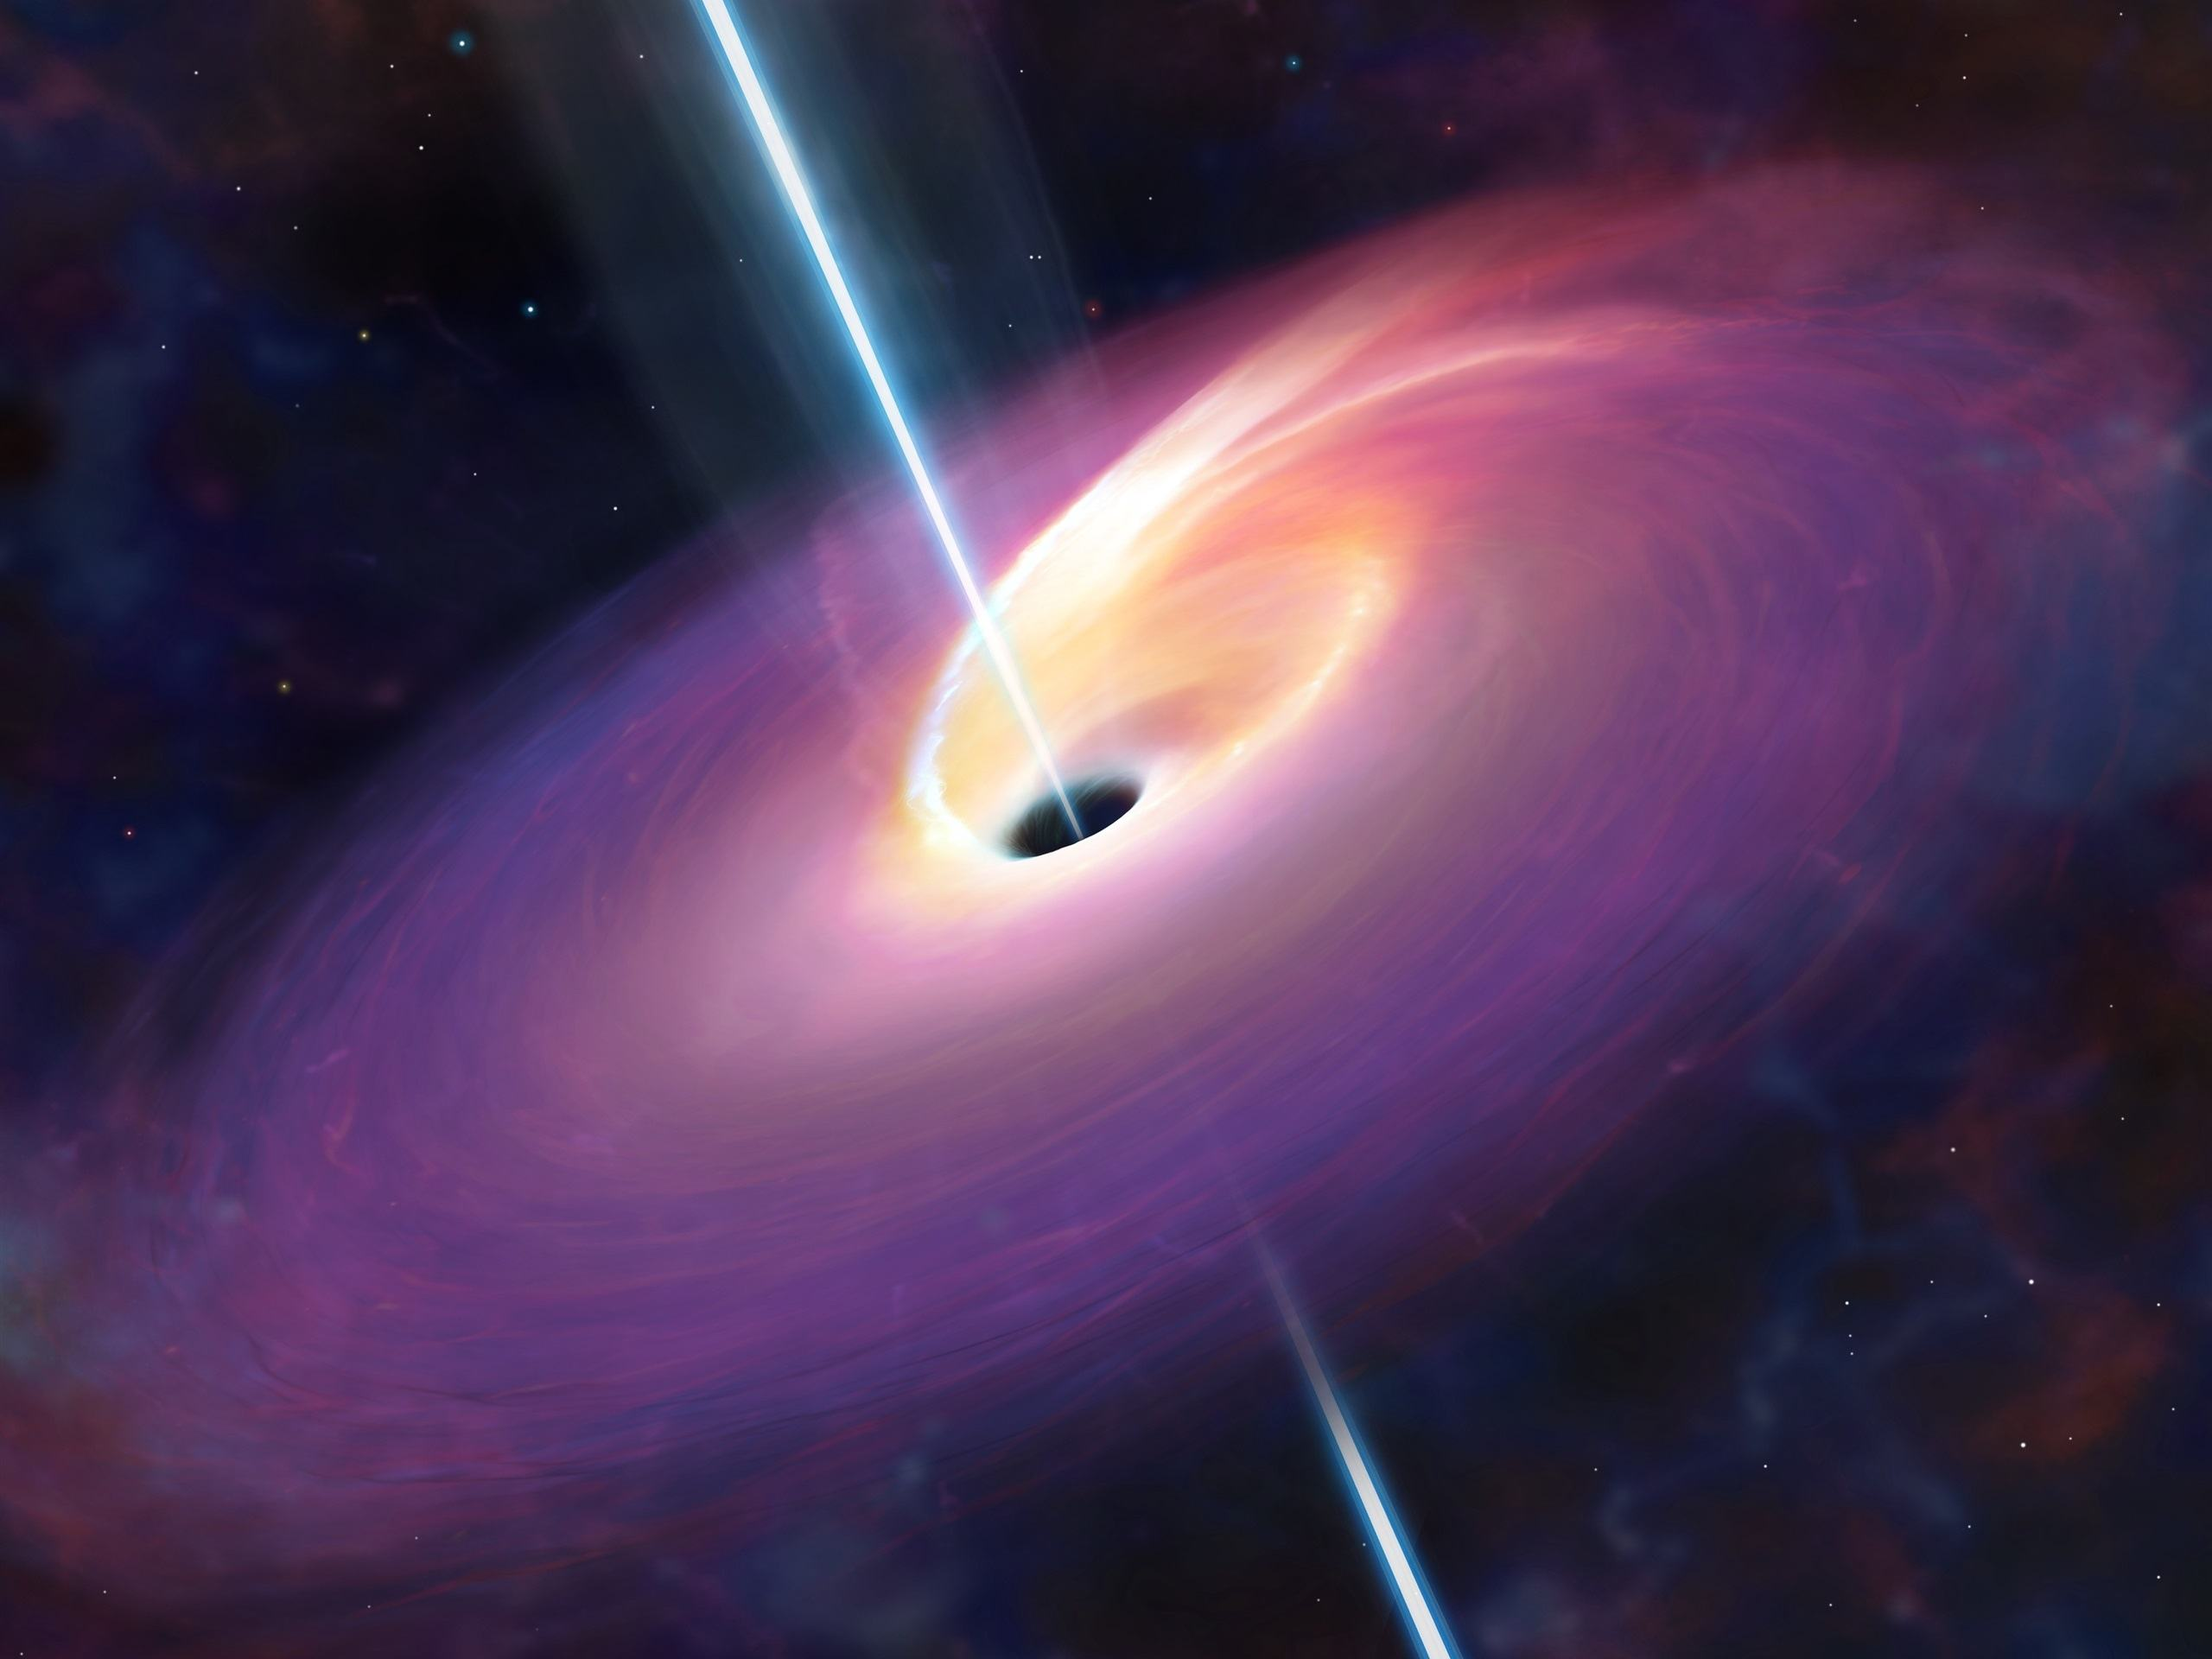
\includegraphics[width = 0.45\textwidth]{images/blackhole.jpeg}
    }
    \hfill
    \subfloat[黑洞4。]{
        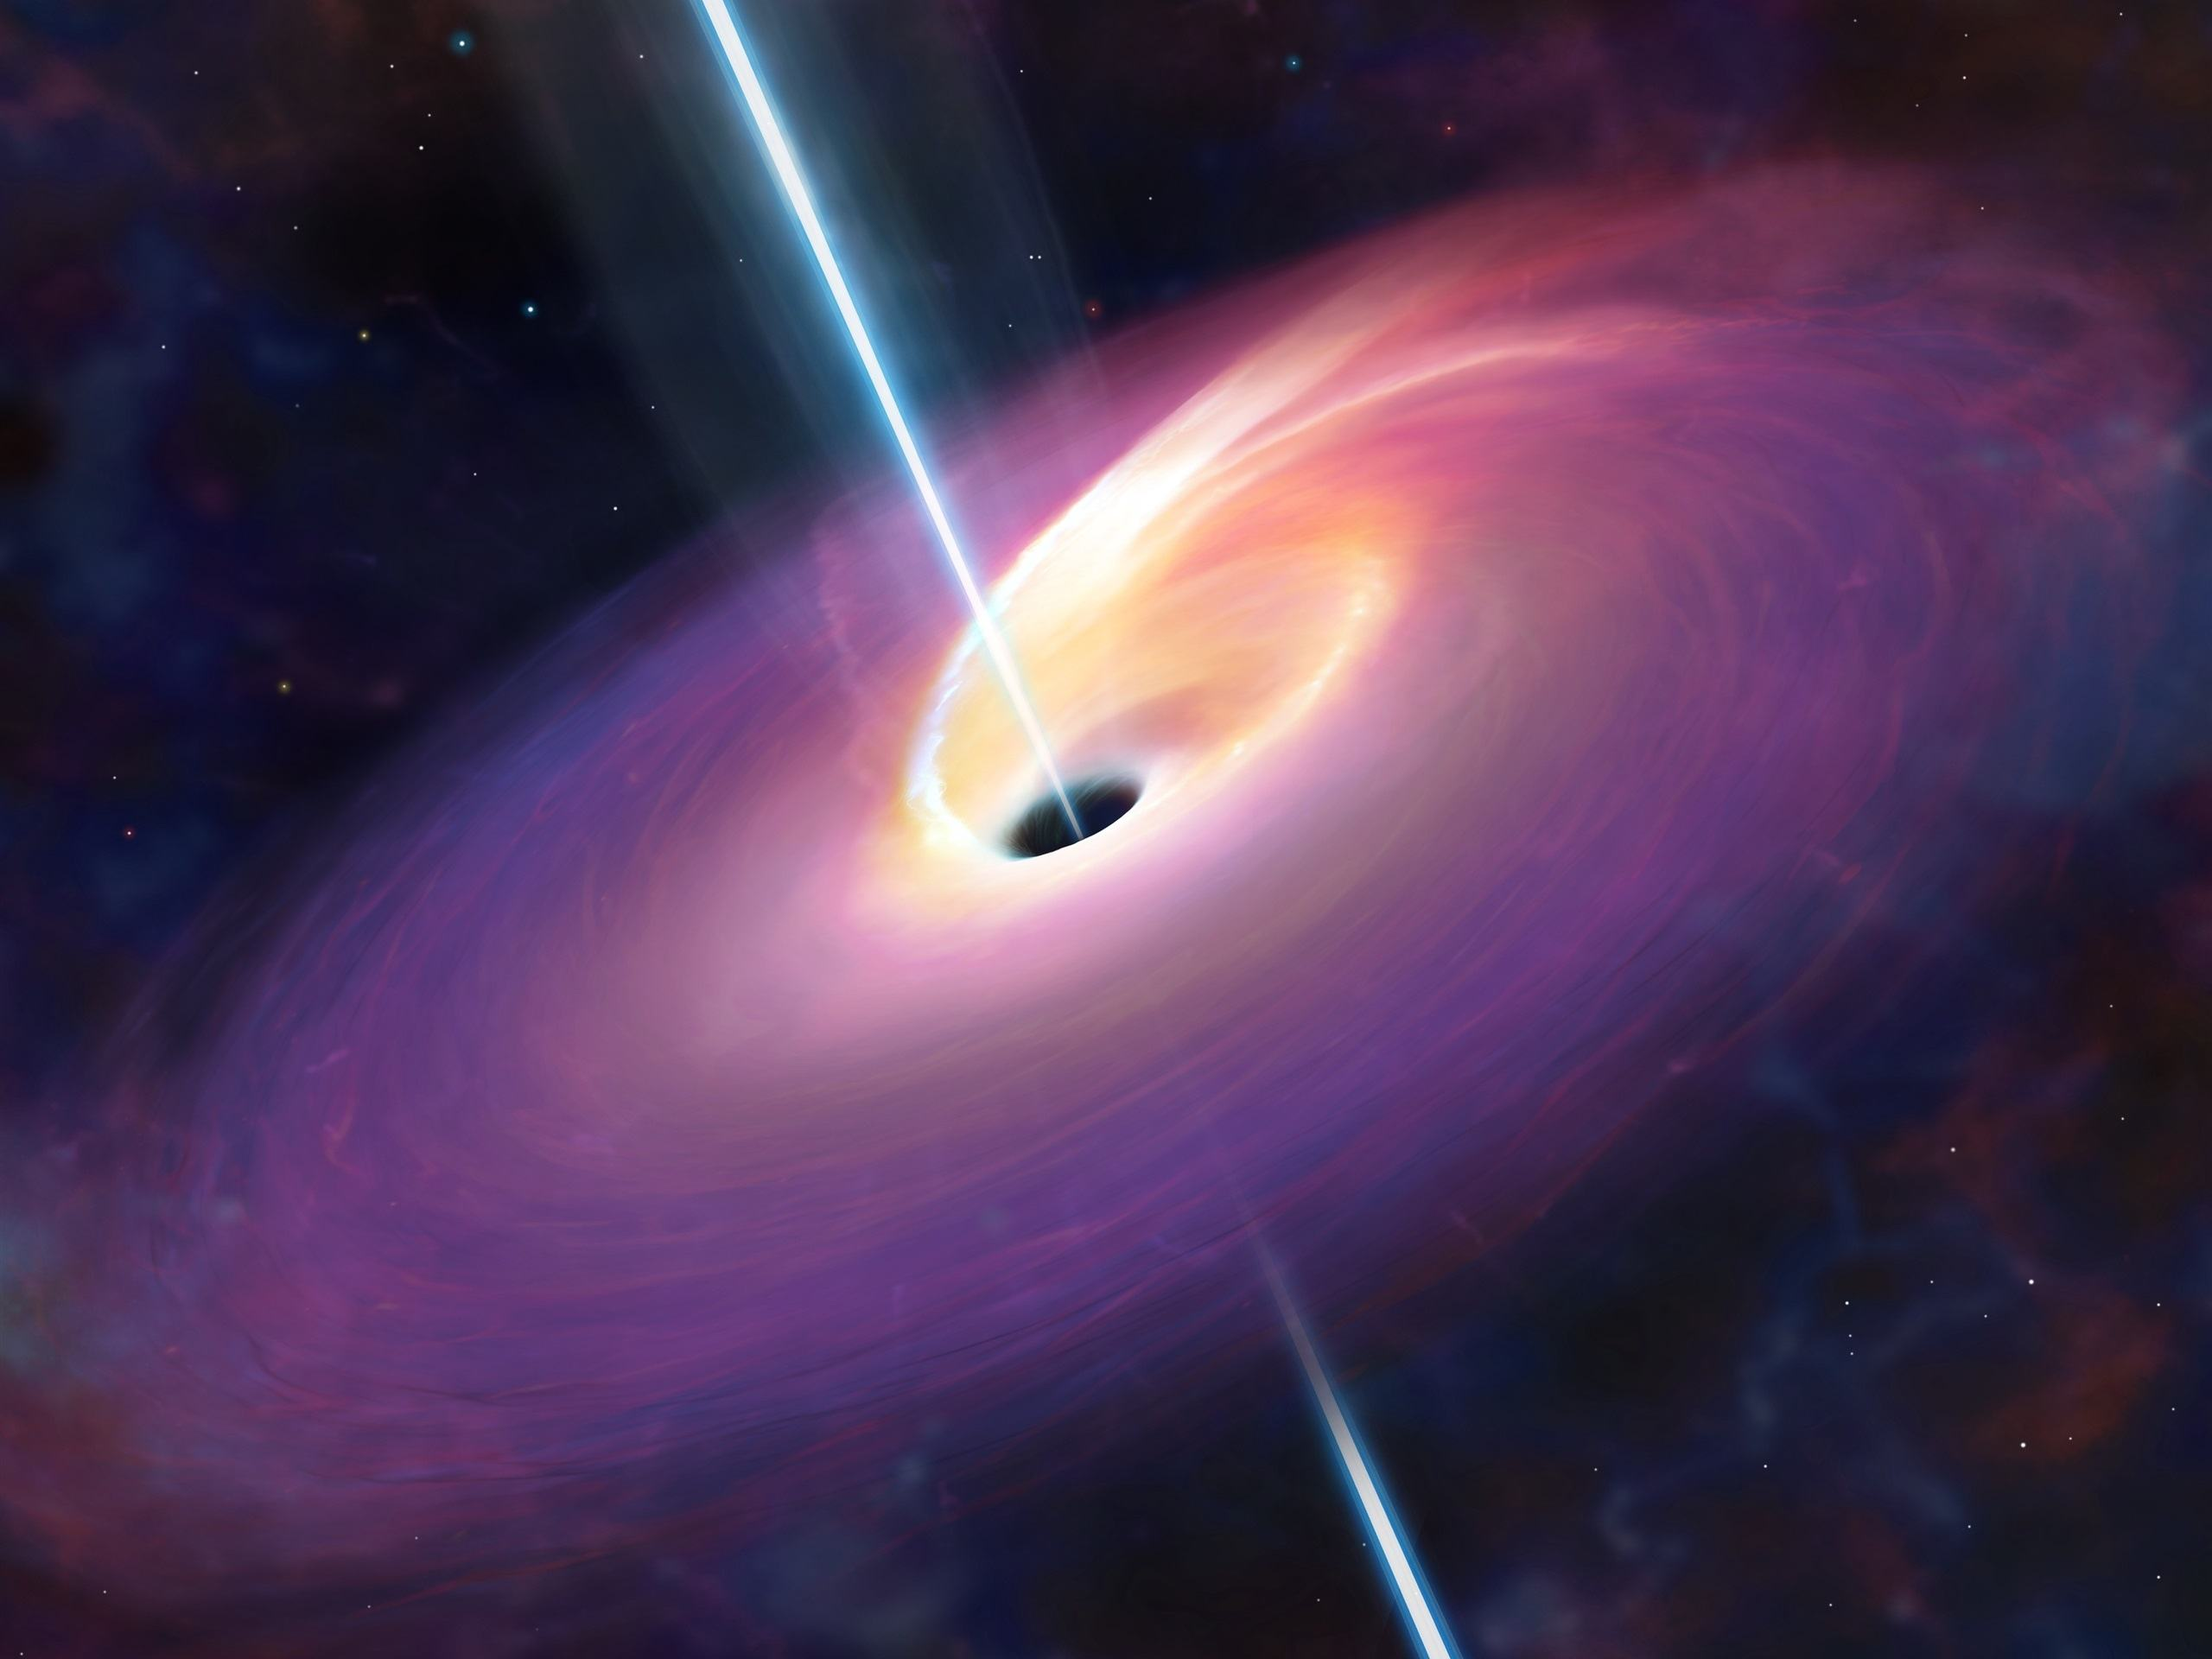
\includegraphics[width = 0.45\textwidth]{images/blackhole.jpeg}
    }
    \caption{多个黑洞}
    \label{fig:blackhole2}
\end{figure*}

图\ref{fig:blackhole2}是多个黑洞图片并列。

\section{表格}

\par \textbf{注意,表格的标题在上面。}

\begin{table}[!ht]
\centering
\caption{一个表的实例}
\label{tab:tabobj}
    \begin{tabular}{cccccc}
        \toprule
        序号 & 姓名 & 性别 & 年龄 & 身高/cm & 体重/kg \\
        \midrule
        1 & 张三 & M & 16 & 163 & 50 \\
        2 & 王红 & F & 15 & 159 & 47 \\
        3 & 李二 & M & 17 & 165 & 52 \\
        \bottomrule
    \end{tabular}
\end{table}

\par 表\ref{tab:tabobj}是一个实例。

\section{简单的数学公式和定理}

\begin{sthm}[定理~\thethm~(存在性定理)]
    $\Gamma\Theta\Lambda\Xi\Pi\alpha\beta\gamma\delta$
\end{sthm}

\begin{thm}
\label{thm:alpha}
    xxxxx
\end{thm}

\begin{equation}
\label{eq:alpha}
    \alpha=\sqrt[n]{\Re}.
\end{equation}
\par 定理\ref{thm:alpha},公式\ref{eq:alpha}。

\section{参考文献}

默认的参考文献引用方法是$\backslash$cite\{\}~\cite{broder1997resemblance,broder1997syntactic},也可以使用非上标的引用形式$\backslash$norcite\{\}~\norcite{broder1997resemblance}。


\section{伪代码实例}

\subsection{使用algorithmic包}

\begin{algorithm}[!ht]
\caption{algorithmic示例}
\begin{algorithmic}[1] %[1] 能够显示行号
    \REQUIRE $n \geq 1$                  %输入条件
    \ENSURE $Sum = 1 + \cdots + n$       %输出
    \STATE $Sum \leftarrow 0$            %\STATE 命名演示
    \IF {$n < 1$}                        %条件语句
        \PRINT {Input Error}                 %打印语句
    \ELSE
        \FOR {$i = 0$ to n}          %FOR循环结构
            \STATE $Sum = Sum + i$\\
            \STATE $i = i + 1$
        \ENDFOR
    \ENDIF
    \RETURN Sum
\end{algorithmic}
\end{algorithm}

% \subsection{使用algorithm2e包}

% \begin{algorithm}[H]
% \caption{algorithm2e示例}
%     \SetAlgoLined
%     \KwData{this text}
%     \KwResult{how to write algorithm with \LaTeX2e }
%     initialization\;
%     \While{not at end of this document}{
%         read current\;
%         \eIf{understand}{
%             go to next section\;
%             current section becomes this one\;
%             }{
%             go back to the beginning of current section\;
%         }
%     }
% \end{algorithm}

% \begin{algorithm}
% \DontPrintSemicolon
% \KwData{$G=(X,U)$ such that $G^{tc}$ is an order.}
% \KwResult{$G’=(X,V)$ with $V\subseteq U$ such that $G’^{tc}$ is an
% interval order.}
% \Begin{
%     $V \longleftarrow U$\;
%     $S \longleftarrow \emptyset$\;
%     \nl\While{$S \neq \emptyset$}{\label{InRes1}
%     \nlset{REM} remove $x$ from the list of $T$ of maximal index\;\label{InResR}
%     \lnl{InRes2}\While{$|S \cap ImSucc(x)| \neq |S|$}{
%     \For{$ y \in S-ImSucc(x)$}{
%         \{ remove from $V$ all the arcs $zy$ : \}\;
%     \For{$z \in ImPred(y) \cap Min$}{
%         remove the arc $zy$ from $V$\;
%         $NbSuccInS(z) \longleftarrow NbSuccInS(z) - 1$\;
%         move $z$ in $T$ to the list preceding its present list\;
%         \{i.e. If $z \in T[k]$, move $z$ from $T[k]$ to
%         $T[k-1]$\}\;
%     }
%     $NbPredInMin(y) \longleftarrow 0$\;
%     $NbPredNotInMin(y) \longleftarrow 0$\;
%     $S \longleftarrow S - \{y\}$\;
%     $AppendToMin(y)$\;
%     }
%     }
%     $RemoveFromMin(x)$\;
%     }
% }
% \caption{IntervalRestriction\label{IR}}
% \end{algorithm}

\section{脚注}

脚注示例\footnote{这是脚注示例。}。



%% 结论
\chapter{结论}\thispagestyle{main}

结论整篇论文。


%% 结论
\chapter{结论}\thispagestyle{main}

结论整篇论文。


%% 攻读学位期间发表的论文
\include{chapter/paper}

%% 参考文献引入
%% 暨大参考文献设置
% \bibliographystyle{thubib}
% 参考文献设置-GB
\bibliographystyle{gbt7714-2005}
\bibliography{bib/refs}

%% 致谢
\chapter*{致\texorpdfstring{\qquad}{} 谢}\addcontentsline{toc}{chapter}{致谢}
\thispagestyle{main}
感谢Yongtao Zhou学长的前期工作,感谢622实验室及朋友们的帮助和支持。

%% 加入\newpage能使最后一页也有页眉
\newpage
\end{document}